% !TeX program = lualatex
% !BIB program = biber
% Lualatex is important to render Fira fonts; with pdflatex it's just the regular one
% ratio 16:9 -- https://tex.stackexchange.com/questions/14336/

\documentclass[12pt,aspectratio=169,handout]{beamer}
% \documentclass[12pt,aspectratio=169]{beamer}


% adjust for 16:9
% https://tex.stackexchange.com/questions/354022/modifying-the-margins-of-all-slides-in-beamer
\setbeamersize{text margin left=0.3cm,text margin right=4.5cm} 

%\usepackage{xcolor}

%%% better TOC
\usetheme[subsectionpage=progressbar]{metropolis}

% name in footer
\setbeamertemplate{frame numbering}{\insertframenumber ~ | Dr.\ Ivan Habernal}

% blocks with background globally
\metroset{block=fill}

% adjust the background to be completely white
\setbeamercolor{background canvas}{bg=white}

% typeset mathematics on serif
\usefonttheme[onlymath]{serif}

% better bibliography using biber as backend
\usepackage[natbib=true,backend=biber,style=authoryear-icomp,maxbibnames=30,maxcitenames=9,uniquelist=false,giveninits=true,doi=false,url=false,dashed=false,isbn=false]{biblatex}
% shared bibliography
\addbibresource{bibliography.bib}
% disable "ibid" for repeated citations
\boolfalse{citetracker}

\definecolor{76abdf}{RGB}{118, 171, 223}

\setbeamercolor{frametitle}{bg=76abdf, fg=white}

\usepackage{xspace}


% for derivatives, https://tex.stackexchange.com/a/412442
\usepackage{physics}

\usepackage{tikz}
\usetikzlibrary{matrix, positioning}
\usetikzlibrary{angles,quotes} % for angles
\usetikzlibrary{backgrounds} % background
\usetikzlibrary{decorations.pathreplacing} % curly braces
\usetikzlibrary{calligraphy}
\usetikzlibrary{calc} % for neural nets

% for plotting functions
\usepackage{pgfplots}
\usepgfplotslibrary{dateplot}

% sub-figures
\usepackage{caption}
\usepackage{subcaption}

% book tabs
\usepackage{booktabs}


% show TOC at every section start
\AtBeginSection{
	\frame{
		\vspace{2em}
		\sectionpage
		\hspace*{2.2em}\begin{minipage}{10cm}
			\tableofcontents[currentsection]
		\end{minipage}
	}
}

% argmin, argmax
\usepackage{amsmath}
\DeclareMathOperator*{\argmax}{arg\!\max}
\DeclareMathOperator*{\argmin}{arg\!\min}

% bold math
\usepackage{bm}



\title{EACL 2023 Tutorial on Privacy-Preserving NLP}
\subtitle{Block 2a, Part 1: Defence with formal guarantees}
\date{May 6, 2023}
\author{Dr.\ Ivan Habernal}
\institute{Trustworthy Human Language Technologies  \hfill 
\includegraphics[height=.8cm]{img/logo-trusthlt.pdf} \\
Department of Computer Science\\
Technical University of Darmstadt \hfill \texttt{www.trusthlt.org} }
%\titlegraphic{\hfill }

\begin{document}

\maketitle


% This block will introduce differential privacy, a mathematical framework for privacy protection \citep{Dwork.Roth.2013}. We will explain the typical setup (why this privacy approach has `differential' in its title) and the formal definitions. Then we will address some basic DP mechanisms and show their NLP applications. This part will involve a few mathematical proofs, but our aim is to make it low-barrier and accessible to a very broad audience.

\section{Differential privacy: Setup and terminology}

\begin{frame}{Trusted curator and dataset}
	
The basic settings: A \textbf{trusted curator} holds a \textbf{database} or \textbf{dataset} (i.e., a table) where

\begin{itemize}
	\item Each entry is linked to a single person
	\item Each person in the dataset is linked to a single entry
\end{itemize}

In other words, the rows are completely independent

\begin{table}
	\begin{tabular}{lrll}
		\toprule
		Name & Income & Last facebook post & ... \\
		\midrule
		Alice & 60,000 & "I hate my job, ..." & ... \\
		Bob & 90,000 & "Spending time with my ..." & ...\\
		... & ... & ... & ...\\
		\bottomrule
	\end{tabular}
\end{table}

\end{frame}

\begin{frame}{Datasets formally}
	
\begin{table}
	\begin{tabular}{lrll}
		\toprule
		Name & Income & Last facebook post & ... \\
		\midrule
		Alice & 60,000 & "I hate my job, ..." & ... \\
		Bob & 90,000 & "Spending time with my ..." & ...\\
		... & ... & ... & ...\\
		\bottomrule
	\end{tabular}
\end{table}

\begin{block}{Dataset $x$ with $n$ individuals as a $n$-tuple}
$$
x = (x_1, x_2, \ldots, x_n)
$$
\end{block}

Note: Many different notations, e.g., $D$, $X$, ...

$x_1$ corresponds to Alice, $x_2$ to Bob, etc.

\begin{tikzpicture}[overlay, remember picture] 
\node at (current page.north east)[anchor = north east, text width=4cm, yshift=-1.3cm] {\scriptsize \fullcite{Vadhan.2017} \par};
\end{tikzpicture}

\end{frame}


\begin{frame}{Neighboring datasets}

\begin{block}{Definition of neighboring datasets}
Neighboring datasets $x$ and $x'$ differ on one row
\end{block}

\begin{itemize}
	\item Variant 1: $x$ and $x'$ have the same size ($|x| = |x'|$), one person is replaced
	\item Variant 2: $|x'| = |x| \pm 1$, one person is removed or added
\end{itemize}


These two options will not protect the same thing.

\begin{itemize}
	\item Variant 1: will protect the value of the record
	\item Variant 2: will also protect the presence of the record in the data
\end{itemize}

\begin{tikzpicture}[overlay, remember picture] 
\node at (current page.north east)[anchor = north east, text width=4cm, yshift=-1.3cm] {\scriptsize \fullcite{Desfontaines.Pejo.2020} \par};
\end{tikzpicture}


\end{frame}


\begin{frame}{Some examples of neighboring datasets $x$ and $x'$ (Variant 2)}
	
\begin{table}
	\begin{tabular}{lrll}
		\toprule
		Alice & 60,000 & "I hate my job, ..." & ... \\
		Bob & 90,000 & "Spending time with ..." & ...\\
		Charlie & 50,000 & "Feeling great" & ...\\
		\bottomrule
	\end{tabular}
	\caption{Dataset $x$}
\end{table}
\begin{table}
	\begin{tabular}{lrll}
		\toprule
		Bob & 90,000 & "Spending time with ..." & ...\\
		Charlie & 50,000 & "Feeling great" & ...\\
		\bottomrule
	\end{tabular}
	\caption{Dataset $x'$}
\end{table}	
$$|x| = 3, |x'| = 2$$
\end{frame}


\begin{frame}{Some examples of neighboring datasets $x$ and $x'$ (Variant 1)}
	
\begin{table}
	\begin{tabular}{lrll}
		\toprule
		Alice & 60,000 & "I hate my job, ..." & ... \\
		\bottomrule
	\end{tabular}
	\caption{Dataset $x$}
\end{table}
\begin{table}
	\begin{tabular}{lrll}
		\toprule
		Bob & 90,000 & "Spending time with ..." & ...\\
		\bottomrule
	\end{tabular}
	\caption{Dataset $x'$}
\end{table}	
$$|x| = 1, |x'| = 1$$

Note: Dataset of size 1 might look a bit extreme, but it follows the definition and will be useful for local DP.

\end{frame}


\begin{frame}{Query}
An \textbf{analyst} or \textbf{adversary} wants to get information about a dataset $x$

Numerical queries
\begin{itemize}
	\item Counting query: $f(x) \to \mathbb{N}$
	\item Mean query: $f(x) \to \mathbb{R}$
	\item General numerical query: $f(x) \to \mathbb{R}^k$
\end{itemize}
	
Arbitrary queries
\begin{itemize}
	\item $f(x) \to \mathcal{Y}$
\end{itemize}
Transformation of the dataset $x$ to any object
	
\end{frame}


\begin{frame}{Example of numeric queries}
\begin{table}
	\begin{tabular}{lrll}
		\toprule
		Alice & 60,000 & "I hate my job, ..." & ... \\
		Bob & 90,000 & "Spending time with ..." & ...\\
		Charlie & 50,000 & "Feeling great" & ...\\
		\bottomrule
	\end{tabular}
	\caption{Dataset $x$}
\end{table}	

\begin{itemize}
	\item Counting query: How many person? $f(x) = 3$
	\item Mean query: Mean income? $f(x) = 6.667$
	\item General numerical query: Histogram of word counts in all Facebook posts: $f(x) = \{\text{my}= 5, \text{the} = 4, \ldots\}$
	\item Arbitrary query: Get copy of Facebook posts $f(x) = (\text{"I hate my job, ..."}, \ldots)$
\end{itemize}

	
\end{frame}

\begin{frame}{Further example queries}
	\begin{table}
		\begin{tabular}{lrll}
			\toprule
			Alice & 60,000 & "I hate my job, ..." & ... \\
			Bob & 90,000 & "Spending time with ..." & ...\\
			Charlie & 50,000 & "Feeling great" & ...\\
			\bottomrule
		\end{tabular}
		\caption{Dataset $x$}
	\end{table}	

\begin{itemize}
	\item Return Facebook posts $f(x) = (\text{"I hate my job, ..."}, \ldots)$
	\item Use the income as a predicted variable $y_i$, use the Facebook text of $x_i$ as an input to a given neural network for income prediction, run a forward pass and backprop, and return the gradient: $f(x) = \left( \pdv{E}{w_1} = 0.02, \pdv{E}{w_2} = -24.9, \ldots \right)$
\end{itemize}

	
\end{frame}


\begin{frame}{Pure differential privacy}

The trusted curator \textbf{randomizes} the query result

\begin{itemize}
	\item Counting query: How many person? $f(x) = 3 + \text{value drawn from a certain probability distribution}$
\end{itemize}

This is called a (randomized) \textbf{mechanism} (algorithm) $\mathcal{M}$ (or $\mathcal{M}(f(x))$, $\mathcal{M}(x)$, $\mathcal{M}(f, x)$, etc.)

\begin{block}{What pure differential privacy guarantees ($\varepsilon \geq 0$)}
For every pair of neighboring datasets $x, x'$ and for any output $y \in \mathcal{Y}$ of $\mathcal{M}$ and query $f$
$$
\frac{
\Pr \left[ \mathcal{M}(f(x)) = y  \right]
}{
\Pr \left[ \mathcal{M}(f(x')) = y  \right]
}
\leq \exp(\varepsilon)
$$
\end{block}

	
\end{frame}

\begin{frame}{Pure $(\varepsilon, 0)$ differential privacy}
	
\begin{block}{What pure differential privacy guarantees ($\varepsilon \geq 0$)}
	For every pair of neighboring datasets $x, x'$ and for any output $y \in \mathcal{Y}$ of $\mathcal{M}$ and query $f$
	$$
	\frac{
		\Pr \left[ \mathcal{M}(f(x)) = y  \right]
	}{
		\Pr \left[ \mathcal{M}(f(x')) = y  \right]
	}
	\leq \exp(\varepsilon)
	$$
\end{block}

Privately querying a dataset $x$ with Alice and dataset $x'$ without Alice will give me two results --- and probabilities of these two results must be similar up to factor $\exp(\varepsilon)$

Why probabilities $\Pr$? Because of the randomness in $\mathcal{M}$	
\end{frame}

\section{Basic DP mechanisms}

\begin{frame}{Laplace mechanism for numeric queries}

PDF of the Laplace distribution:
$$
\mathrm{Lap}(x; \mu, b) = \frac{1}{2b} \exp \left( - \frac{| x - \mu |}{b} \right)
$$
To privatize a query output by adding noise from the Laplace distribution, we need to know the \textbf{scale} $b$.

\begin{block}{Global sensitivity $\Delta f$}
What is the maximum difference of the query $f$ for any two neighboring datasets $x, x'$
$$
\Delta f = \max_{x, x'} | f(x) - f(x')|
$$
\end{block}
	
\end{frame}

\begin{frame}{Global sensitivity and Laplace mechanism}

\begin{example}
Sensitivity of the counting query $\Delta f = 1$
\end{example}

The scale $b$ of the Laplace noise is then proportional to the sensitivity and privacy budget $\varepsilon$:
$$
b = \frac{\Delta f}{\varepsilon}
$$


\begin{block}{The Laplace mechanism}
$$
\mathcal{M_{\mathrm{Lap}}}(f(x)) = f(x) + z \qquad
z \sim \textrm{Lap}(\mu = 0; b = \Delta f / \varepsilon)
$$
\end{block}

\end{frame}


\begin{frame}{Example of the Laplace mechanism for a counting query}

Laplace mechanism satisfies $(\varepsilon)$-DP\footnote{
Step-by-step proof at	https://blog.ivanhabernal.com/2020-11-10-detailed-proof-of-laplace-mechanism-in-differential-privacy.html}

\begin{figure}
	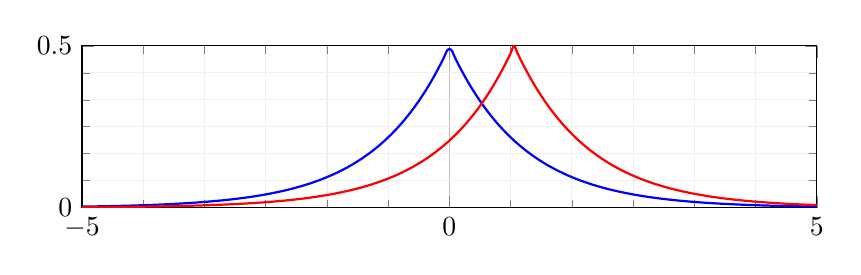
\begin{tikzpicture}
	
	\begin{axis}[
	xmin = -5, xmax = 5,
	ymin = 0, ymax = 0.5,
	xtick distance = 5,
	ytick distance = 0.5,
	grid = both,
	minor tick num = 5,
	major grid style = {lightgray},
	minor grid style = {lightgray!25},
	width = 0.9\textwidth,
	height = 0.30\textwidth,
	legend pos = north west
	]
	
	\addplot[
	domain = -5:5,
	samples = 200,
	smooth,
	thick,
	blue,
	] {(1/2*1) * exp( - abs(x) / 1)};
	
		\addplot[
	domain = -5:5,
	samples = 200,
	smooth,
	thick,
	red,
	] {(1/2*1) * exp( - abs(x - 0.88) / 1)}; % no idea why x-1 produces a wrong plot :(
	
	\end{axis}
	\end{tikzpicture}
	\caption{Laplace PDFs for two means: $0$ and $1$ corresponding to the max difference of two datasets for counting queries with $\Delta f = 1$. Plotted for $\varepsilon = 1.0$.}
\end{figure}



\end{frame}

\begin{frame}{Exponential mechanism for discrete outputs}

Given some arbitrary range (set) $\mathcal{R}$, the \textbf{exponential mechanism} is defined to some utility function $u: x \times \mathcal{R} \to \mathbb{R}$, which maps database/output pairs to utility scores


We prefer that the mechanism outputs some element of $\mathcal{R}$ with the maximum possible utility score

\begin{example}
$x$ is a word, $\mathcal{R}$ is a set of words, the utility $u$ is some similarity or word $x$ and words in $\mathcal{R}$, e.g., a similarity of word embeddings (the higher, the better)
\end{example}

\begin{tikzpicture}[overlay, remember picture] 
\node at (current page.north east)[anchor = north east, text width=4cm, yshift=-1.3cm] {\scriptsize Sampling from soft-max in language generation: \fullcite{Mattern.et.al.2022.Findings} \par};
\end{tikzpicture}

\end{frame}

\begin{frame}{Exponential mechanism is $\varepsilon$-DP}
Sensitivity of the utility score $\Delta u$ is defined
$$
\Delta u = \max_{\forall r \in \mathcal{R}, x, x'} |u(x, r) - u(y, r)|
$$

The exponential mechanism\footnote{
For a step-by-step proof see https://blog.ivanhabernal.com/2021-06-30-detailed-proof-of-exponential-mechanism.html
} $\mathcal{M}_E(x, u, \mathcal{R})$ selects and outputs an element $r \in \mathcal{R}$ with probability proportional to
$$\exp \left( \frac{\varepsilon \cdot u(x,r)}{2\Delta u}\right)$$

\end{frame}

\section{Approximate DP}

\begin{frame}{Privacy loss random variable}
The mechanism $\mathcal{M(f(x))}$ is in fact a \textbf{random variable} parametrized by the query $f$ and the dataset $x$, and as such it has a certain \textbf{probability distribution}

is this even important?

$$
\frac{
	\Pr \left[ \mathcal{M}(f(x)) = y  \right]
}{
	\Pr \left[ \mathcal{M}(f(x')) = y  \right]
}
\leq \exp(\varepsilon)
$$


\end{frame}


\section{Application of Differential Privacy in NLP}

\subsection{Publishing models trained with DP}

\begin{frame}{XXX}
	
\end{frame}

\subsection{Synthetic data generation with DP-trained models}

\begin{frame}{XXX}
	
\end{frame}

\subsection{Word-level privacy}

\begin{frame}{XXX}
	
\end{frame}

\subsection{Data publishing with local differential privacy}

\begin{frame}{XXX}
	
\end{frame}



\section*{Recap}

\begin{frame}{Take aways}
	
\begin{itemize}
	
	\item XXX
\end{itemize}
	
\end{frame}



\begin{frame}{License and credits}

	\begin{columns}
		\begin{column}{0.7\textwidth}
			Licensed under Creative Commons Attribution-ShareAlike 4.0 International (CC BY-SA 4.0)
		\end{column}
		\begin{column}{0.2\textwidth}
			
\includegraphics[width=0.9\linewidth]{img/cc-by-sa-icon.pdf}
		\end{column}
	\end{columns}
	
	\bigskip
	
	Credits
	
	\begin{scriptsize}
		
		Ivan Habernal
		
		Content from ACL Anthology papers licensed under CC-BY \url{https://www.aclweb.org/anthology}
		
	\end{scriptsize}
	
\end{frame}



\end{document}

